\documentclass[12pt]{article}
% \usepackage[margin=1.25in]{geometry}
\usepackage[inner=2.0cm,outer=2.0cm,top=2.5cm,bottom=2.5cm]{geometry}
\usepackage{color}
\usepackage{graphicx}
\usepackage{amssymb}
\usepackage{amsmath}
\usepackage{amsthm}
\usepackage{bm}
\usepackage{hyperref}
\usepackage{multirow}
\usepackage{mathtools}
\usepackage{enumerate}
\usepackage{ctex}

\newcommand{\homework}[5]{
	\pagestyle{myheadings}
	\thispagestyle{plain}
	\newpage
	\setcounter{page}{1}
	\noindent
	\begin{center}
		\framebox{
			\vbox{\vspace{2mm}
				\hbox to 6.28in { {\bf KRP \hfill #2} }
				\vspace{6mm}
				\hbox to 6.28in { {\Large \hfill #1 \hfill} }
				\vspace{6mm}
				\hbox to 6.28in { {\it Instructor: {\rm #3} \hfill Name: {\rm #4}, StudentId: {\rm #5}}}
				\vspace{2mm}}
		}
	\end{center}
	% \markboth{#4 -- #1}{#4 -- #1}
	\vspace*{4mm}
}


\begin{document}
\large
	%==========================Put your name and id here==========================
	\homework{Homework 2}{Spring 2023}{YiZheng Zhao}{张运吉}{211300063}
    \paragraph{Question 1. Closure under Disjoint Union}~{}
    \\
    
    Let $\mathcal{K}=<\mathcal{T}, \mathcal{A}>$ be a $\mathcal{ALC}$ knowledge base, $(\mathcal{I}_{v})_{v \in \Omega}$ a family of models of $\mathcal{K}$. \par
    The extend the notion of disjoint union to individual names is as follow: \par
    \begin{itemize}
        \item $\Delta^{\mathcal{J}} = \{ (d,v)| v \in \Omega \text{ and } d \in \Delta^{\mathcal{I}_v} \}$
        \item $A^{\mathcal{J}} = \{ (d,v)| v \in \Omega \text{ and } d \in A^{\mathcal{I}_v} \}$ for all $A \in \mathbf{C}$
        \item $r^{\mathcal{J}} = \{ ((d,v), (e,v)) | v \in \Omega \text{ and } (d, e) \in r^{\mathcal{I}_v} \}$ for all $r \in \mathbf{R}$
        \item $a^{\mathcal{J}} = (a^{\mathcal{I}_{v}}, v)$
    \end{itemize} \par
    Now we prove that : for any family
    $(\mathcal{I}_{v})_{v \in \Omega}$ of models of an ALC-knowledge base $\mathcal{K}$, the disjoint union $\mathcal{J} = \biguplus_{v \in \Omega}$ is also a model of $\mathcal{K}$.
    Use proof by contradiction: \par
    If $\mathcal{J}$ is not a model of $\mathcal{T}$, then there exists a $\text{GCI: } C \sqsubseteq D$, such that $C^{\mathcal{J}} \not\subseteq D^{\mathcal{J}}$, which means there exists a element $(d, v)$ in $C^{\mathcal{J}}$, but not in $D^{\mathcal{J}}$, so there exist a $\mathcal{I}_v$ such that $d \in C^{\mathcal{I}_v}, d\not\in D^{\mathcal{I}_v}$. And what is contradictory to $\mathcal{I}_v$ is a model of $\mathcal{T}$. So $\mathcal{J}$ is a model of $\mathcal{T}$. \par
    If $\mathcal{J}$ is not a model of $\mathcal{K}$ \par
    case 1: there exists a $\text{Assertion: } a : A$, such that $a^{\mathcal{J}} \not\in A^{\mathcal{J}}$, which means there exist a $\mathcal{I}_v$ such that $a^{\mathcal{I}_v} \not\in A^{\mathcal{I}_v}$. And what is contradictory to $\mathcal{I}_v$ is a model of $\mathcal{K}$. \par
    case 2: there exists a $\text{Assertion: } (a, b) : r$, such that $((a^{\mathcal{J}}, v), (b^{\mathcal{J}}, v)) \not\in r^{\mathcal{J}}$, which means there exist a $\mathcal{I}_v$ such that $(a^{\mathcal{I}_v}, a^{\mathcal{I}_v}) \not\in r^{\mathcal{I}_v}$. And what is contradictory to $\mathcal{I}_v$ is a model of $\mathcal{K}$. \par
    So $\mathcal{J}$ is a model of $\mathcal{K}$. \par
    To sum up, $\mathcal{J} = \biguplus_{v \in \Omega}$ is also a model of $\mathcal{K}$.
    
    \paragraph{Question 2. Closure under Disjoint Union}~{}
    \\

    $C \sqsubseteq_{\mathcal{T}} D \Longrightarrow  C \sqsubseteq_{\mathcal{K}} D $: \par
	If $C \sqsubseteq_{\mathcal{T}} D$, then $C^{\mathcal{I}} \subseteq D^{\mathcal{I}}$ hold for all models $\mathcal{I}$ of $\mathcal{T}$. For any model $\mathcal{J}$ of $\mathcal{K}$, it must a modle  of $\mathcal{T}$, so we know  $C^{\mathcal{J}} \subseteq D^{\mathcal{J}}$ holds for all model $\mathcal{J}$ of $\mathcal{K}$,
    so $C \sqsubseteq_{\mathcal{K}} D$ \par
    $C \sqsubseteq_{\mathcal{K}} D \Longrightarrow  C \sqsubseteq_{\mathcal{T}} D $: \par
    If $C \not\sqsubseteq_{\mathcal{T}} D$, then there exists a model $\mathcal{I}_0$ of $\mathcal{T}$, but $C^{\mathcal{I}_0} \not\subseteq D^{\mathcal{I}_0}$, because $\mathcal{K}$ is consistent, we can extend $\mathcal{I}_0$ such that $\mathcal{I}_0$ became a model of $\mathcal{K} = <\mathcal{T}, \mathcal{A}>$.\par
    Then we construct a disjoint union $\mathcal{J} = \mathcal{I}_0 \cup \mathcal{I}_1$. ($\mathcal{I}_1$ is model of $\mathcal{K}$ and $C^{\mathcal{I}_1} \subseteq D^{\mathcal{I}_1}$). According to the conclusion of Q1, $\mathcal{J}$ is also a model of $\mathcal{K}$, but $C^{\mathcal{J}} \not\subseteq D^{\mathcal{J}}$. And what is contradictory to $C \sqsubseteq_{\mathcal{K}} D$.
    So we get $C \sqsubseteq_{\mathcal{T}} D$.
    \paragraph{Question 3. Finite Model Property (fmp)}~{}
    \\
    \begin{enumerate}
    \item[(1)] True.\par
    According to Finite Model Property, $C$ has a finite model, which means there exists model $\mathcal{I}$ of $\mathcal{T} \text{ s.t. } |C^{\mathcal{I}}| \geq 1$. \par
    Let $\mathcal{I}_m = \biguplus_{v \in \{ 1, \cdots, m \}}\mathcal{I}$, so $|C^{\mathcal{I}_m}| \geq m$.
    \item[(2)]  False.\par
    Here's a counter-example: Let $C = \top$, $\mathcal{T} = \{ A \sqsubseteq \exists r.\lnot A, \lnot A  \sqsubseteq \exists r.A \}$ and $m = 1$. \par
    If the conclusion holds, then there exists only one element in $\Delta^{\mathcal{I}}$, because: $\Delta^{\mathcal{I}} = A^{\mathcal{I}} \cup \lnot A^{\mathcal{I}}$. \par
    case 1: $A^{\mathcal{I}} = \emptyset$, so $\exists r. A = \emptyset$, according to the second GCI in $\mathcal{T}$, $\lnot A = \emptyset$, and then $\Delta^{\mathcal{I}} = A^{\mathcal{I}} \cup \lnot A^{\mathcal{I}} = \emptyset$.And what is contradictory. \par
    case 2: $\lnot A^{\mathcal{I}} = \emptyset$, so $\exists r. \lnot A = \emptyset$, according to the first GCI in $\mathcal{T}$, $ A = \emptyset$, and then $\Delta^{\mathcal{I}} = A^{\mathcal{I}} \cup \lnot A^{\mathcal{I}} = \emptyset$.And what is contradictory. \par 
    So : $A^{\mathcal{I}} \neq \emptyset \text{ and } \lnot A^{\mathcal{I}} \neq \emptyset$, which means $|\Delta^{\mathcal{I}} = A^{\mathcal{I}} \cup \lnot A^{\mathcal{I}}| \geq 2$.\par
    It doesn't hold if the condition $|C^{\mathcal{I}_m}| \ge m$ is replaced by $|C^{\mathcal{I}_m}| = m$.
\end{enumerate}
    \paragraph{Question 4. Bisimulation over Filtration}~{}
    \\

    False.\par
    Let $C = A$ and $\mathcal{T} = \{ \exists r.\top \sqsubseteq \top \}$, so $S = \operatorname{sub}(C) \cup \operatorname{sub}(\mathcal{T}) = \{ \top, A, \exists r.\top \}$.\par
    \begin{figure}[htbp]
		\centering 
		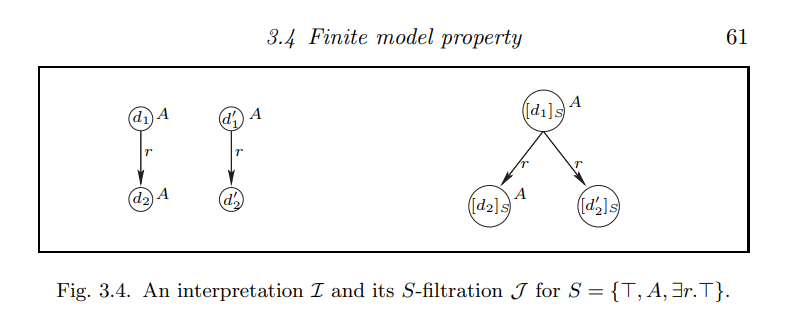
\includegraphics[width=1.0\textwidth,height=0.5\textwidth]{hw2_4.png}
	\end{figure} 
    $[d_1]_S=\{d_1, d_1^{'}\}, [d_2]_S=\{d_2\}, [d_2^{'}]_S=\{d_2^{'}\}$\par
    we can see that the relation $\rho = \{ (d, [d]) | d \in \Delta^{\mathcal{I}} \}$ is not a bisimmulation between $\mathcal{I}$ and $\mathcal{J}$.

    \paragraph{Question 5. Bisimulation within the Same Interpretation}~{}
    \\

    \begin{enumerate}
        \item [(1)]
        \begin{itemize}
            \item $d_1 \approx_\mathcal{I} d_2$ implies there is a bisimulation $\rho$ on $\mathcal{I}$ such that $d \rho e$,which means \par
            \begin{equation}
                d_1\in A^\mathcal{I} \text{ iff } d_2\in A^\mathcal{I}
            \end{equation}
             for all $d_1 \in \Delta^{\mathcal{I}}$, $d_2 \in \Delta^{\mathcal{I}} \text{ and } A \in C$.\par
            \item $d_1\approx_\mathcal{I}d_2$ implies there is a bisimulation $d_1 \rho d_2$, due to the bisimualtion, $(d_1,d_1^{'})\in r^\mathcal{I}$ implies there exists $d_2^{'} \in \Delta^\mathcal{I}$ such that \par
            \begin{equation}
                d_1^{'}\,\rho\, d_2^{'} \text{ and } (d_2,d_2^{'})\in r^\mathcal{I}
            \end{equation}
            for all $d_1, d_1^{'}, d_2 \in \Delta^{\mathcal{I}} \text{ and }r\in \mathbf{R}$.\par
            \item $d_1\approx_\mathcal{I}d_2$ implies there is a bisimulation $d_1 \rho d_2$, due to the bisimualtion, $(d_2,d_2^{'})\in r^\mathcal{I}$ implies there exists $d_1^{'} \in \Delta^\mathcal{I}$ such that \par
            \begin{equation}
                d_1^{'}\,\rho\, d_2^{'} \text{ and } (d_1,d_1^{'})\in r^\mathcal{I}
            \end{equation}
            for all $d_1, d_2^{'}, d_2 \in \Delta^{\mathcal{I}} \text{ and }r\in \mathbf{R}$.\par
        \end{itemize}
        So $\thickapprox_{\mathcal{I}}$ is a bisimulation on $\mathcal{I}$. \par
        \item [(2)]
        \begin{itemize}
            \item $d\,\rho\,[d]_{\thickapprox_{\mathcal{I}}}$ implies $d\in A^\mathcal{I}$ iff $[d]_{\thickapprox_{\mathcal{I}}}\in A^\mathcal{J}$ \par
            If $d\in A^\mathcal{I}$, there must be a $[d]_{\thickapprox_{\mathcal{I}}}\in A^\mathcal{J}$ by the definition of filtration. On the contrary, if $[d]_{\thickapprox_{\mathcal{I}}} \in A^\mathcal{J}$, according to the definition, there exists $d' \in [d]_{\thickapprox_{\mathcal{I}}}$ such that $d\approx_{\mathcal{I}}d'$ and $d'\in A^\mathcal{I}$, because $\approx_\mathcal{I}$ is a bisimulation on $\mathcal{I}$, so $d\in A^\mathcal{I}$. Therefore, $d\in A^\mathcal{I}$ iff $[d]_{\thickapprox_{\mathcal{I}}}\in A^\mathcal{J}$. \par
            \item $d\,\rho\, [d]_{\thickapprox_{\mathcal{I}}}$ and $(d,d')\in r^\mathcal{I}$ implies there exists $[d']_{\thickapprox_{\mathcal{I}}}\in \Delta^\mathcal{J}$, $d'\, \rho \, [d']_{\thickapprox_{\mathcal{I}}}$ and $([d]_{\thickapprox_{\mathcal{I}}}, [d']_{\thickapprox_{\mathcal{I}}})\in r^\mathcal{J}$. \par
            If $(d,d')\in r^\mathcal{I}$, there must be $[d']_{\thickapprox_{\mathcal{I}}}\in \Delta^\mathcal{J}$. Because of the third property of the definition of a filtration, there is $([d]_{\thickapprox_{\mathcal{I}}},[d']_{\thickapprox_{\mathcal{I}}}) \in r^\mathcal{J}, \;\ d\in \left[d\right]_{\thickapprox_{\mathcal{I}}} ,\; d'\in\left[d'\right]_{\thickapprox_{\mathcal{I}}} \, \left(d,d'\right)\in r^\mathcal{I}\;$. \par
            \item $(d, [d]_{\thickapprox_{\mathcal{I}}}) \in \rho$ and $([d]_{\thickapprox_{\mathcal{I}}}, [e]_{\thickapprox_{\mathcal{I}}}) \in r^{\mathcal{J}}$ implies there is $d' \in [d]_{\thickapprox_{\mathcal{I}}}$, $e' \in [e]_{\thickapprox_{\mathcal{I}}}$ with $(d', e') \in r^{\mathcal{I}}$. \par
            Because $d \in [d]_{\thickapprox_{\mathcal{I}}}$, we can know $d \thickapprox_{\mathcal{I}} d'$. And $\thickapprox_{\mathcal{I}}$ is a bisimulation on $\mathcal{I}$, which implies the existence of $e \in \Delta^{\mathcal{I}}$ such that
$e \thickapprox_{\mathcal{I}} e'$ and $(d, e) \in r^{\mathcal{I}}$
So we can know
$(e, [e]_{\thickapprox_{\mathcal{I}}}) \in \rho$ and $(d, e) \in r^{\mathcal{I}}$
for all $d \in \Delta^{\mathcal{I}}$, $[d]_{\thickapprox_{\mathcal{I}}}, [e]_{\thickapprox_{\mathcal{I}}} \in \Delta^{\mathcal{J}}$, and $r \in \mathbf{R}$.
\par 

        \end{itemize}
        So we show that $\rho = \{ (d, [d]_{\thickapprox_{\mathcal{I}}}) | d \in \Delta^{\mathcal{I}} \}$ is a bisimulation between $\mathcal{I}$ and $\mathcal{J}$.
        \item [(3)]
        If $\mathcal{I}$ is a model of an $\mathcal{ALC}$-concept $C$ w.r.t an $\mathcal{ALC}$-TBox $\mathcal{T}$, then $C^{\mathcal{I}} \neq \emptyset$.

If $d \in C^{\mathcal{I}}$, because there is a bisimulation between $\mathcal{I}$ and $\mathcal{J}$, so $[d]_{\thickapprox_{\mathcal{I}}} \in C^{\mathcal{J}}$ according to  bisimulation invariance of $\mathcal{ALC}$.

It is easy to see that $\mathcal{J}$ is a model of $\mathcal{T}$. Let $D \sqsubseteq E$ be a GCI in $\mathcal{T}$ and $[d]_{\thickapprox_{\mathcal{I}}} \in D^{\mathcal{J}}$. By bisimulation invariance, $d \in D^{\mathcal{I}}$ and  $d \in E^{\mathcal{I}}$ because $\mathcal{I}$ is a model of $\mathcal{T}$.Therefore $[d]_{\thickapprox_{\mathcal{I}}} \in E^{\mathcal{J}}$.

So $\mathcal{J}$ is a model of an $\mathcal{ALC}$-concept $C$ w.r.t an $\mathcal{ALC}$-TBox $\mathcal{T}$.
        \item [(4)]
        Because we can't  get the bound of the $|\Delta^{\mathcal{J}}|$.\par
        For example,  $\mathcal{T} = \{A\sqsubseteq \exists r.B, B \sqsubseteq \exists r.A, A\sqcup B\sqsubseteq \exists s.\top \}$. \par
\begin{figure}[htbp]
    \centering
    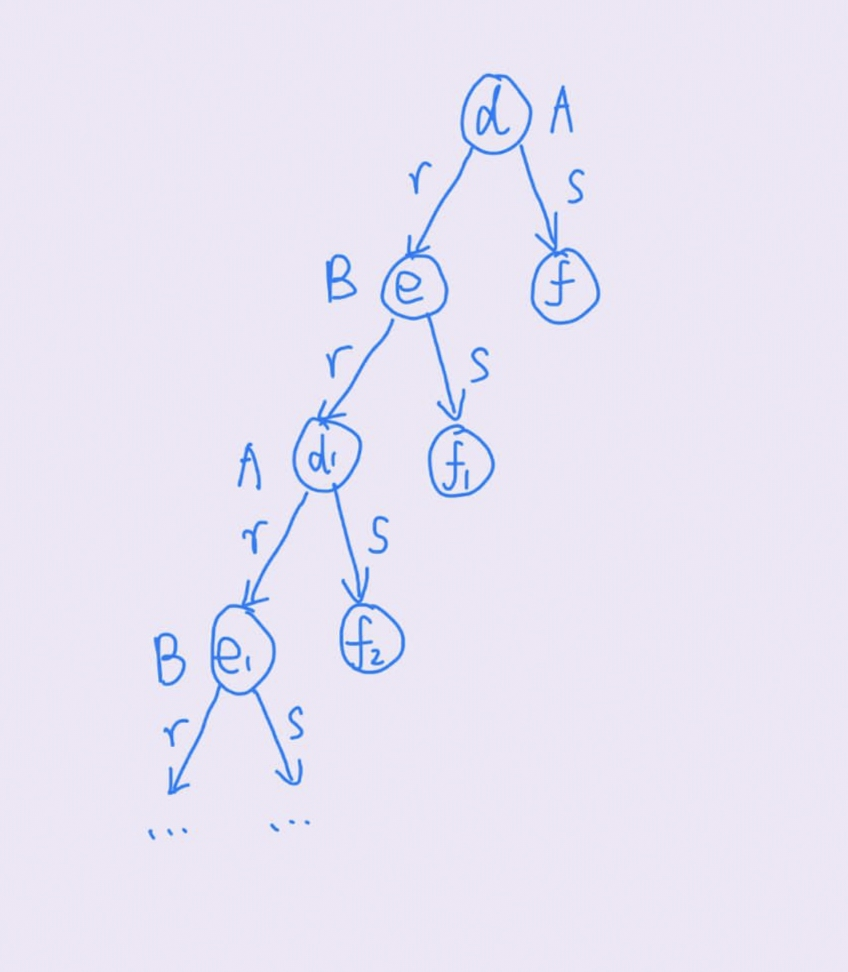
\includegraphics[width=0.8\textwidth,height=0.5\textwidth]{4.jpg}
\end{figure}
According the graph, we can find a Interpretation $\mathcal{J}$, but it appearently is not finite.\par
    \end{enumerate}

    \paragraph{Question 6. Unravelling}~{}
    \\

    See the following figure:\par
    \begin{figure}[htbp]
        \centering
        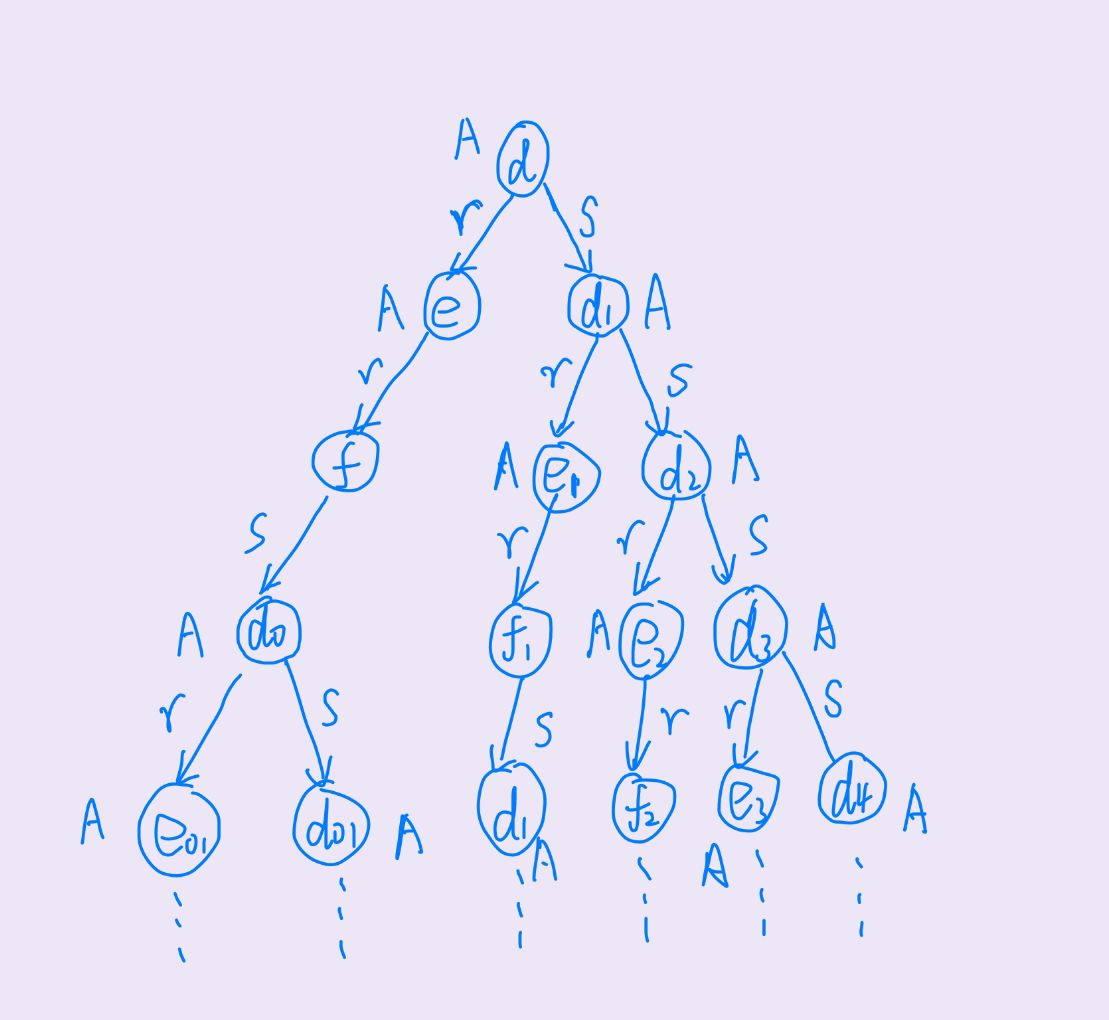
\includegraphics[width=0.8\textwidth,height=0.4\textwidth]{hw2_6.jpg}
    \end{figure}

    \paragraph{Question 7. Tree Model Property (tmp)}~{}
    \\

    False. \par
    For example, if $\mathcal{K} = <\mathcal{T},\mathcal{A}>$ and $\mathcal{T} = \emptyset, \mathcal{A} = \{ a:A, b:B,(a,b):r,(b,a):r\}$. For every model  $\mathcal{I}$ of $\mathcal{K}$, $a^\mathcal{I}$ and $b^\mathcal{I}$ are two distinguish elements, and $(a^\mathcal{I},b^\mathcal{I}), (b^\mathcal{I},a^\mathcal{I})\in r^\mathcal{I}$. Therefore, the model always have a cycle $a\rightarrow b\rightarrow a$, which means it is not a tree model.\par
    \paragraph{Question 8. Tableau Algorithm}~{}
    \\

    $\mathcal{A}_0 = \{ (b,a): r, (a,b): r, (a,c): s, (c,b):s, a: \exists s.A,  b: \forall r.((\forall s.\lnot A)\sqcup (\exists r.B)), $\par
    $c: \forall s.(B \sqcap (\forall s.\bot)) \}$ \par
    for $a: \exists s.A$, apply the $\exists$-rule: \par
    $$\mathcal{A}_1 = \mathcal{A}_0 \cup \{ (a,d): s, d: A \}$$\par
    for $b: \forall r.((\forall s.\lnot A)\sqcup (\exists r.B))$, apply the $\forall$-rule:\par
    $$\mathcal{A}_2 = \mathcal{A}_1 \cup \{ a: (\forall s.\lnot A)\sqcup (\exists r.B) \}$$\par
    for $c: \forall s.(B \sqcap (\forall s.\bot))$, apply the $\forall$-rule:\par
    $$\mathcal{A}_3 = \mathcal{A}_2 \cup \{ b: B \sqcap (\forall s.\bot) \}$$\par
    for $b: B \sqcap (\forall s.\bot)$, apply the $\cup$-rule:\par
    $$\mathcal{A}_4 = \mathcal{A}_3 \cup \{ b: B, b: \forall s.\bot \}$$\par
    for $a: (\forall s.\lnot A)\sqcup (\exists r.B)$, apply $\sqcup$-rule:\par
    case 1: $$\mathcal{A}_5 = \mathcal{A}_4 \cup \{ a: \forall s.\lnot A \}$$\par
    \quad\quad for $a: \forall s.\lnot A$, apply the $\forall$-rule:\par
    \quad\quad $$\mathcal{A}_{51} = \mathcal{A}_5 \cup \{ c: \lnot A, d: \lnot A \}$$ \par
    \quad\quad because $\mathcal{A}_{51}$ contains a clash $d: A$ and $d: \lnot A$, so fail.\par
    case 2: $$\mathcal{A}_5 = \mathcal{A}_4 \cup \{ a: \exists r.B\}$$\par
    \quad\quad there is no rule is applicable and $\mathcal{A}_5$ does not contains clash.\par
    So, we have done. $\mathcal{A}$ is consistent.
    \begin{figure}[htbp]
		\centering
		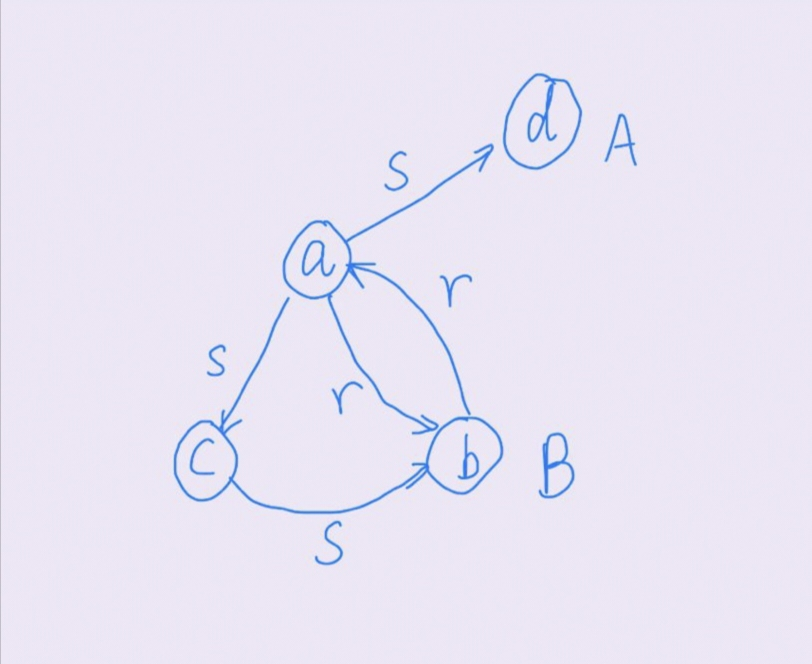
\includegraphics[width=0.8\textwidth,height=0.5\textwidth]{hw2_8.jpg}
	\end{figure} 
    \paragraph{Question 9. Extension of Tableau Algorithm}~{}
    \\

    Define the NNF of $\rightarrow$-constructer:$\lnot(C\rightarrow D) \equiv C\sqcap \lnot D$ ,they are semantically equivalent because $(C \to D)^{\mathcal{I}}  = \{ x \in \Delta^{\mathcal{I}} | x \in \Delta^{\mathcal{I}} \setminus C^{\mathcal{I}} \text{ or } x \in D^{\mathcal{I}} \}  = (\lnot C \sqcup D)^{\mathcal{I}}$.\par
    \begin{enumerate}
        \item[(1)] The deterministic $\rightarrow $-rule:\par
        Termination: \par 
        The property termination still holds. \par
        Let $m = |\operatorname{sub}(\mathcal{A})|$. \par
        a.After applying application, it will add a new assertion of the form $a: C$ and $C \in \operatorname{sub}(\mathcal{A})$. So for any individual name $a$, there can be at most m rule applications
        adding a concept assertion of the form $a : C$ and $\operatorname{con}_{\mathcal{A}}(a) \le m$.
        \par 
        b. A new individual name is added to A only when the $\exists$-rule is
        applied to an assertion of the form $a : C$ with $C$ an existential
        restriction (a concept of the form $\exists \text{r.D}$), and for any individual
        name each such assertion can trigger the addition of at most one
        new individual name. As there can be no more than m different
        existential restrictions in A, a given individual name can cause
        the addition of at most m new individual names, and the outdegree of each tree in the forest-shaped ABox is thus bounded by
        m.\par
        c. With the same original proof, the depth of each tree in the forest-shaped ABox is bounded by $m$.\par
        There properties ensure that there is a bound on the size of the ABox that can be constructed via
rule applications, and thus a bound on the number of recursive applications of expand. \par
        Soundness: \par
        The property soundness does not holds. \par
        For example, $\mathcal{A} = \{ a: (C \sqcup D) \to E, a: C,a: \lnot E  \}$, because $a: C \sqcup D \not \in \mathcal{A}$,we could not use the deterministic rule, so there is no rule could be applicated to it and there is no clash, therefore the algorithm would return $\mathcal{A}$ is consistent. But actually the ABox is conflicting semantically.\par
        Completeness: \par
        The property completeness still holds. \par
        Let $\mathcal{A}$ be consistent, and consider a model $\mathcal{I} = <\Delta^{\mathcal{I}}, \cdot^{\mathcal{I}}>$ of A.
Since $\mathcal{A}$ is consistent, it cannot contain a clash.
If $\mathcal{A}$ is complete - since it does not contain a clash - expand simply
returns $\mathcal{A}$ and consistent returns “consistent”. If $\mathcal{A}$ is not complete, then
expand calls itself recursively until $\mathcal{A}$ is complete; each call selects a rule
and applies it. We will show that rule application preserves consistency
by a case analysis according to the type of rule:
\begin{figure}[htbp]
    \centering
    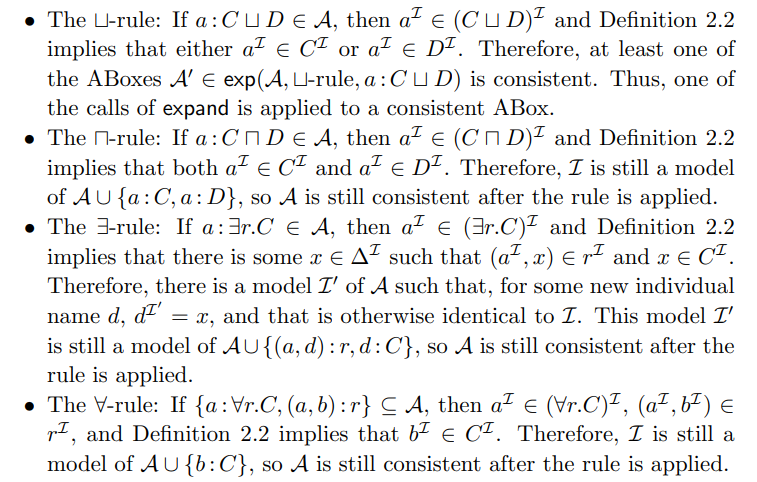
\includegraphics[width=0.8\textwidth,height=0.5\textwidth]{hw9.png}
\end{figure}  \par
We also need to prove $\rightarrow$-rule: If $a: C \to D \in \mathcal{A}$ and $a: C \in \mathcal{A}$, then $a^{\mathcal{I}} \in (C \to D)^{\mathcal{I}}$. So there is $a^{\mathcal{I}} \in \Delta^{\mathcal{I}} \setminus C^{\mathcal{I}}$ or $a^{\mathcal{I}} \in D^{\mathcal{I}}$ according to the semantics of $\to$. Because we have $a^{\mathcal{I}} \in C^{\mathcal{I}}$, so there is $a^{\mathcal{I}} \in D^{\mathcal{I}}$. Therefore, $\mathcal{I}$ is still a model of $\mathcal{A} \cup \{ a: D \}$, so $\mathcal{A}$ is still consistent after applying the rule. \par 
\item[(2)] The nondeterministic $\rightarrow $-rule:\par
Termination: \par
The property termination still holds. The proof is as the same as deterministic case.\par
Soundness: \par
The property soundness still holds. \par
\begin{figure}[htbp]
    \centering
    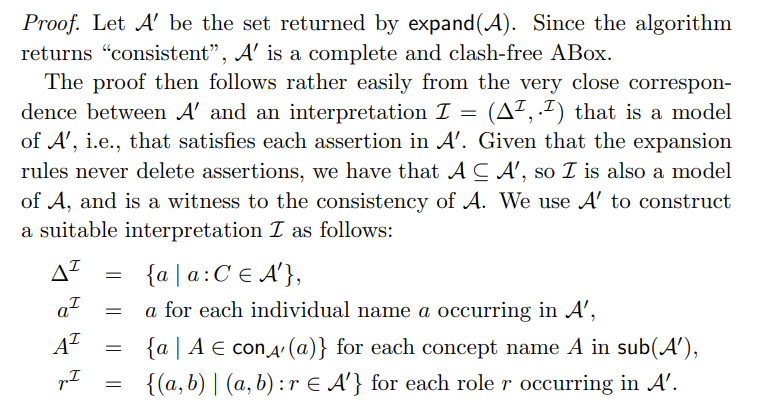
\includegraphics[width=0.8\textwidth,height=0.5\textwidth]{hw92.png}
\end{figure}  \par
The construction of $\mathcal{I}$ means that it trivially satisfies all role assertions in $\mathcal{A}'$.\par
we will show the following property by induction of the structure of concept: \par
if $a: C \in \mathcal{A}'$, then $a^{\mathcal{I}} \in C^{\mathcal{I}}$ \par \newpage
\begin{figure}[htbp]
    \centering
    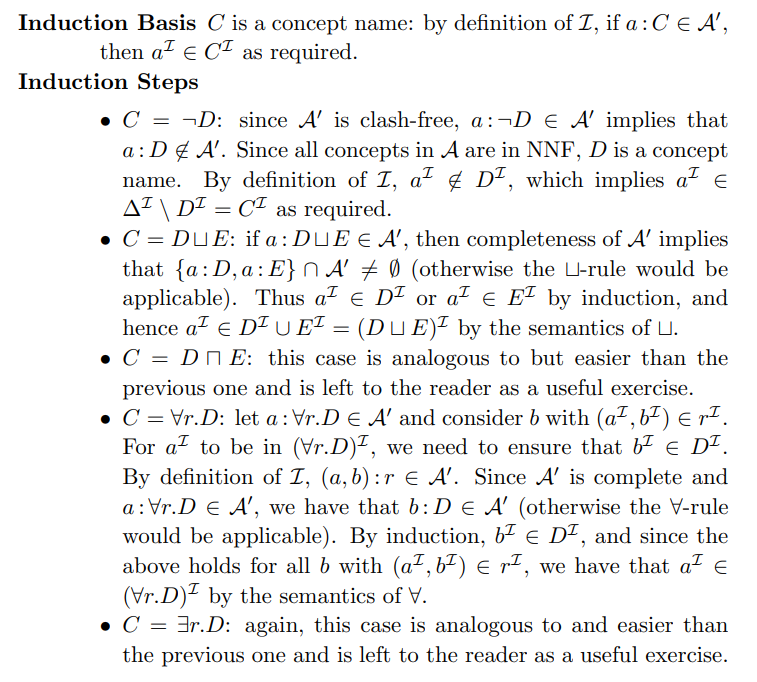
\includegraphics[width=0.8\textwidth,height=0.5\textwidth]{hw91.png}
\end{figure}  \par
we also need to prove the case when $C=D\rightarrow E$: if $a: D \to E \in \mathcal{A}'$, then completeness of $\mathcal{A}'$ implies that $\{ a: E \} \subseteq \mathcal{A}'$ or $\{ a: \dot{\lnot} D \} \subseteq \mathcal{A}'$ (otherwise the nondeterministic $\to$-rule would be applicable). Thus $a^{\mathcal{I}} \in E^{\mathcal{I}}$ or $a^{\mathcal{I}} \in \Delta^{\mathcal{I}} \setminus D^{\mathcal{I}}$ by induction, and hence $a^{\mathcal{I}} \in (\Delta^{\mathcal{I}} \setminus D^{\mathcal{I}}) \cup E^{\mathcal{I}} = (\lnot D \sqcup E)^{\mathcal{I}} = (D \to E)^{\mathcal{I}}$ by the semantics of $\to$.\par
As a consequence, $\mathcal{I}$ satisfies all concept assertions in $\mathcal{A}'$ and thus in $\mathcal{A}$, and it satisfies all role assertions in $\mathcal{A}'$ and thus in $\mathcal{A}$ by definition. Hence $\mathcal{A}$ has a model and thus is consistent.\par
Completeness:\par
The property completeness still holds. \par
The body of the proof is the same as above, we just need to modify it a bit.\par
The nondeterministic $\to$-rule: If $a: C \to D \in \mathcal{A}$, then $a^{\mathcal{I}} \in (C \to D)^{\mathcal{I}}$. Thus $a^{\mathcal{I}} \in \Delta^{\mathcal{I}} \setminus C^{\mathcal{I}}$ or $a^{\mathcal{I}} \in D^{\mathcal{I}}$ by the semantics of $\to$. Therefore, at least one of the ABoxes $\mathcal{A}' \in \exp (\mathcal{A}, \text{nondeterministic } \to \text{-rule}, a: C \to D)$ is consistent. Thus, one of the calls of expand is applied to a consistent ABox.\par
\end{enumerate}
    
    \paragraph{Question 10. Modification of Tableau Algorithm}~{}
    \\
    
    We firstly extend the definition of a clash: for some individual name $a$, and for some concept $C$, $\{ a: C, a: \lnot C \} \subseteq \mathcal{A}$, or for some individual names $a$ and $b$, and for some role names $r$ and $s$, $\{ (a, b): r, (a, b): s \} \subseteq \mathcal{A}$ and $\{ \text{disjoint}(r, s) \} \subseteq \mathcal{T}$.\par
    Define $\sqsubseteq$-rule: \par
    \begin{itemize}
        \item Condition: $(a, b): r\in \mathcal{A}, r\sqsubseteq s\in\mathcal{T} $ and $(a, b): s \not \in \mathcal{A}$.\par
        \item Action: $\mathcal{A} \rightarrow \mathcal{A} \cup \{ (a, b): s \}$. \par
    \end{itemize}
    Now, we show that the algorithm remains terminating, sound, and complete. For the sake of simplicity, we will follow the proof in Question 9 and modify it if necessary.\par
    \begin{itemize}
        \item Termination. \par
        Because the number of individual names is bounded, so the number of new role assertions added by $\sqsubseteq$-rule is bounded. \par
        \item Soundness. \par
        Let $\mathcal{A}'$ be the set return by $\text{expand}(\mathcal{A})$. Since the algorithm returns "consistent", $\mathcal{A}'$ is a complete and clash-free ABox. \par
        If $\text{disjoint}(r,s)\in \mathcal{T}$, $r^{\mathcal{I}} \cap s^{\mathcal{I}} \neq \emptyset$, which means there exists $(a,b)\in r^\mathcal{I}$ and $(a,b)\in s^\mathcal{I}$. And then we can conclude $(a,b):r, (a,b):s\in \mathcal{A}'$ which is a clash, therefore $r^\mathcal{I}\cap s^\mathcal{I} = \emptyset$. \par
        If $r\sqsubseteq s\in \mathcal{T}$ but there is $(a,b)\in r^\mathcal{I}, (a,b)\not\in s^\mathcal{I}$. Then by the definition of $\mathcal{I}$, $(a, b): r \in \mathcal{A}'$ but $(a, b): s \not \in \mathcal{A}'$, which means $\mathcal{A}'$ is not a complete ABox. \par
        Therefore, if the consistent($\mathcal{T}$,$\mathcal{A}$) returns "consistent", then ($\mathcal{T}$,$\mathcal{A}$) is consistent.\par
        \item Completeness. \par
        Let $\mathcal{I}$ be a model of ($\mathcal{T}$,$\mathcal{A}$). if $(a,b):r\in\mathcal{A}$, $r\sqsubseteq s\in \mathcal{T}$ and $(a,b)\in r^\mathcal{I}$. Because $\mathcal{I}$ is a model of ($\mathcal{T}$, $\mathcal{A}$), so there must be $(a,b)\in s^\mathcal{I}$. Therefore, $\mathcal{I}$ is also a model of ($\mathcal{T}$, $\mathcal{A} \cup \{(a,b):s\}$), so $\mathcal{A}$ is still consistent after the rule is applied.\par
    \end{itemize}
\end{document}
